\documentclass{extbook}[14pt]
\usepackage{multicol, enumerate, enumitem, hyperref, color, soul, setspace, parskip, fancyhdr, amssymb, amsthm, amsmath, latexsym, units, mathtools}
\everymath{\displaystyle}
\usepackage[headsep=0.5cm,headheight=0cm, left=1 in,right= 1 in,top= 1 in,bottom= 1 in]{geometry}
\usepackage{dashrule}  % Package to use the command below to create lines between items
\newcommand{\litem}[1]{\item #1

\rule{\textwidth}{0.4pt}}
\pagestyle{fancy}
\lhead{}
\chead{Answer Key for Progress Quiz 10 Version C}
\rhead{}
\lfoot{5170-5105}
\cfoot{}
\rfoot{Summer C 2021}
\begin{document}
\textbf{This key should allow you to understand why you choose the option you did (beyond just getting a question right or wrong). \href{https://xronos.clas.ufl.edu/mac1105spring2020/courseDescriptionAndMisc/Exams/LearningFromResults}{More instructions on how to use this key can be found here}.}

\textbf{If you have a suggestion to make the keys better, \href{https://forms.gle/CZkbZmPbC9XALEE88}{please fill out the short survey here}.}

\textit{Note: This key is auto-generated and may contain issues and/or errors. The keys are reviewed after each exam to ensure grading is done accurately. If there are issues (like duplicate options), they are noted in the offline gradebook. The keys are a work-in-progress to give students as many resources to improve as possible.}

\rule{\textwidth}{0.4pt}

\begin{enumerate}\litem{
Choose the equation of the function graphed below.

\begin{center}
    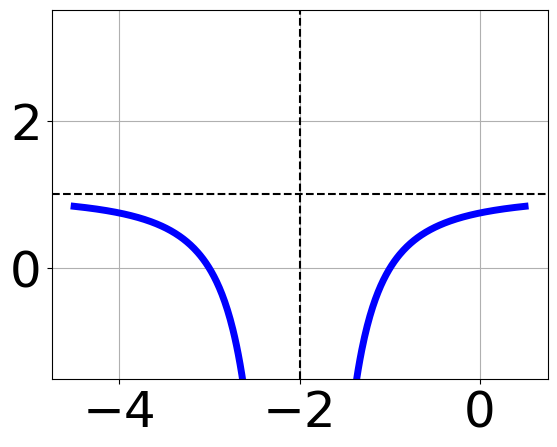
\includegraphics[width=0.5\textwidth]{../Figures/rationalGraphToEquationCopyC.png}
\end{center}


The solution is \( f(x) = \frac{-1}{(x + 2)^2} + 1 \), which is option C.\begin{enumerate}[label=\Alph*.]
\item \( f(x) = \frac{1}{(x - 2)^2} + 1 \)

Corresponds to using the general form $f(x) = \frac{a}{(x+h)^2}+k$ and the opposite leading coefficient.
\item \( f(x) = \frac{-1}{x + 2} + 1 \)

Corresponds to thinking the graph was a shifted version of $\frac{1}{x}$.
\item \( f(x) = \frac{-1}{(x + 2)^2} + 1 \)

This is the correct option.
\item \( f(x) = \frac{1}{x - 2} + 1 \)

Corresponds to thinking the graph was a shifted version of $\frac{1}{x}$, using the general form $f(x) = \frac{a}{(x+h)^2}+k$, and the opposite leading coefficient.
\item \( \text{None of the above} \)

This corresponds to believing the vertex of the graph was not correct.
\end{enumerate}

\textbf{General Comment:} Remember that the general form of a basic rational equation is $ f(x) = \frac{a}{(x-h)^n} + k$, where $a$ is the leading coefficient (and in this case, we assume is either $1$ or $-1$), $n$ is the degree (in this case, either $1$ or $2$), and $(h, k)$ is the intersection of the asymptotes.
}
\litem{
Solve the rational equation below. Then, choose the interval(s) that the solution(s) belongs to.
\[ \frac{8}{-4x + 2} + 2 = \frac{-3}{-32x + 16} \]The solution is \( x = 1.547 \), which is option D.\begin{enumerate}[label=\Alph*.]
\item \( x_1 \in [1, 2.3] \text{ and } x_2 \in [1.83,2.12] \)

$x = 1.547 \text{ and } x = 1.875$, which corresponds to getting the correct solution and believing there should be a second solution to the equation.
\item \( \text{All solutions lead to invalid or complex values in the equation.} \)

This corresponds to thinking $x = 1.547$ leads to dividing by zero in the original equation, which it does not.
\item \( x_1 \in [0.5, 1.2] \text{ and } x_2 \in [1.49,1.64] \)

$x = 0.547 \text{ and } x = 1.547$, which corresponds to getting the correct solution and believing there should be a second solution to the equation.
\item \( x \in [1.55,2.55] \)

* $x = 1.547$, which is the correct option.
\item \( x \in [0.5,1.2] \)

$x = 0.547$, which corresponds to not distributing the factor $-4x + 2$ correctly when trying to eliminate the fraction.
\end{enumerate}

\textbf{General Comment:} Distractors are different based on the number of solutions. Remember that after solving, we need to make sure our solution does not make the original equation divide by zero!
}
\litem{
Determine the domain of the function below.
\[ f(x) = \frac{3}{30x^{2} +10 x -20} \]The solution is \( \text{All Real numbers except } x = -1.000 \text{ and } x = 0.667. \), which is option A.\begin{enumerate}[label=\Alph*.]
\item \( \text{All Real numbers except } x = a \text{ and } x = b, \text{ where } a \in [-1.3, 0.2] \text{ and } b \in [0.2, 1.4] \)

All Real numbers except $x = -1.000$ and $x = 0.667$, which is the correct option.
\item \( \text{All Real numbers except } x = a, \text{ where } a \in [-1.3, 0.2] \)

All Real numbers except $x = -1.000$, which corresponds to removing only 1 value from the denominator.
\item \( \text{All Real numbers except } x = a, \text{ where } a \in [-25.6, -24.6] \)

All Real numbers except $x = -25.000$, which corresponds to removing a distractor value from the denominator.
\item \( \text{All Real numbers except } x = a \text{ and } x = b, \text{ where } a \in [-25.6, -24.6] \text{ and } b \in [22.6, 25.6] \)

All Real numbers except $x = -25.000$ and $x = 24.000$, which corresponds to not factoring the denominator correctly.
\item \( \text{All Real numbers.} \)

This corresponds to thinking the denominator has complex roots or that rational functions have a domain of all Real numbers.
\end{enumerate}

\textbf{General Comment:} Recall that dividing by zero is not a real number. Therefore the domain is all real numbers \textbf{except} those that make the denominator 0.
}
\litem{
Choose the graph of the equation below.
\[ f(x) = \frac{-1}{x - 3} + 1 \]The solution is the graph below, which is option D.
    \begin{center}
        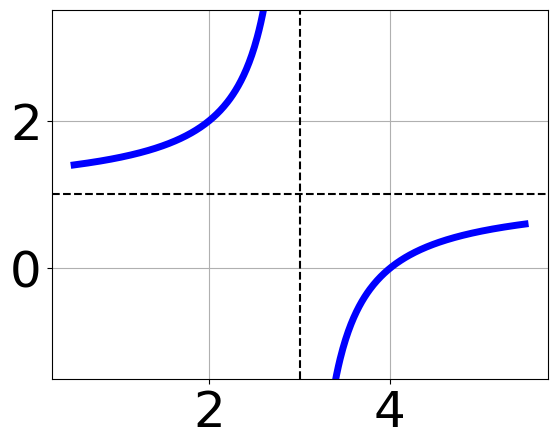
\includegraphics[width=0.3\textwidth]{../Figures/rationalEquationToGraphCopyDC.png}
    \end{center}\begin{enumerate}[label=\Alph*.]
\begin{multicols}{2}
\item 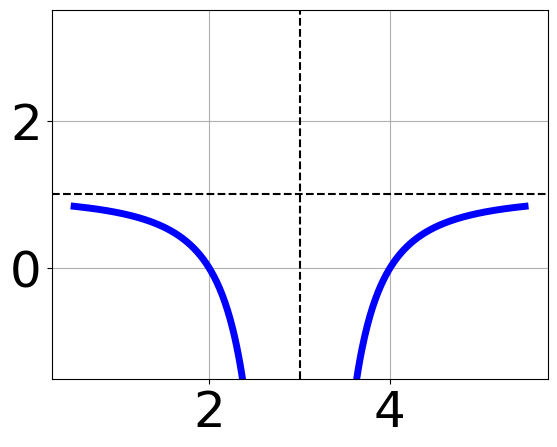
\includegraphics[width = 0.3\textwidth]{../Figures/rationalEquationToGraphCopyAC.png}
\item 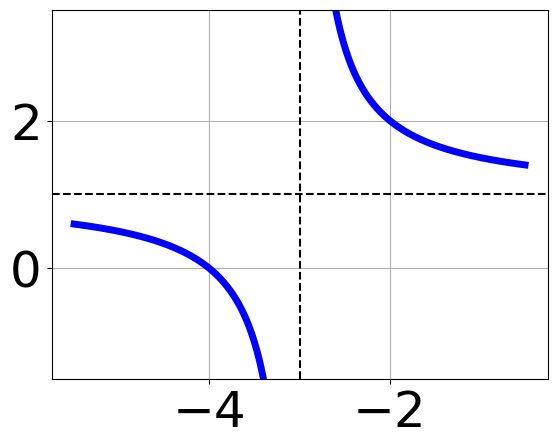
\includegraphics[width = 0.3\textwidth]{../Figures/rationalEquationToGraphCopyBC.png}
\item 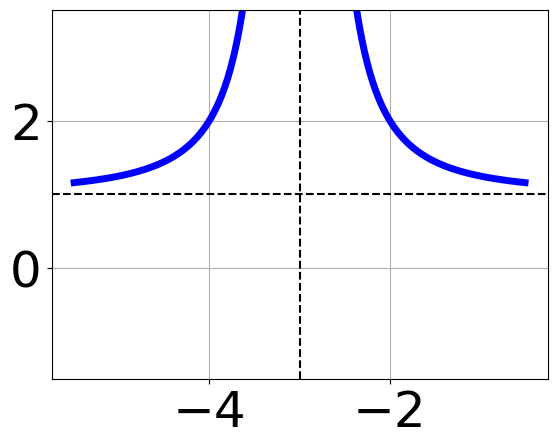
\includegraphics[width = 0.3\textwidth]{../Figures/rationalEquationToGraphCopyCC.png}
\item 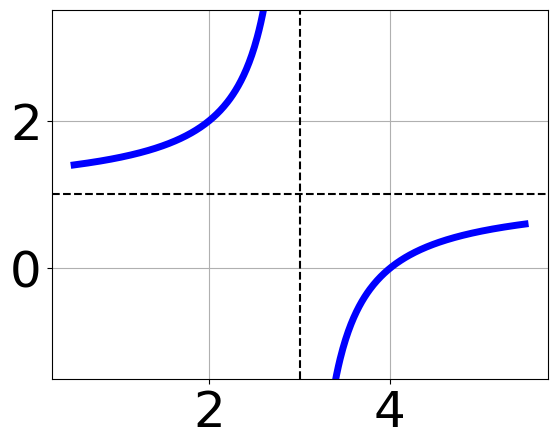
\includegraphics[width = 0.3\textwidth]{../Figures/rationalEquationToGraphCopyDC.png}
\end{multicols}\item None of the above.\end{enumerate}
\textbf{General Comment:} Remember that the general form of a basic rational equation is $ f(x) = \frac{a}{(x-h)^n} + k$, where $a$ is the leading coefficient (and in this case, we assume is either $1$ or $-1$), $n$ is the degree (in this case, either $1$ or $2$), and $(h, k)$ is the intersection of the asymptotes.
}
\litem{
Solve the rational equation below. Then, choose the interval(s) that the solution(s) belongs to.
\[ \frac{7x}{-3x -5} + \frac{-4x^{2}}{-9x^{2} -36 x -35} = \frac{7}{3x + 7} \]The solution is \( \text{There are two solutions: } x = -3.535 \text{ and } x = -0.582 \), which is option D.\begin{enumerate}[label=\Alph*.]
\item \( x \in [-1.9,5] \)


\item \( x_1 \in [-4.3, -2.9] \text{ and } x_2 \in [-2.45,-0.81] \)


\item \( x \in [-3.2,-0.7] \)


\item \( x_1 \in [-4.3, -2.9] \text{ and } x_2 \in [-0.67,1.13] \)

* $x = -3.535 \text{ and } x = -0.582$, which is the correct option.
\item \( \text{All solutions lead to invalid or complex values in the equation.} \)


\end{enumerate}

\textbf{General Comment:} Distractors are different based on the number of solutions. Remember that after solving, we need to make sure our solution does not make the original equation divide by zero!
}
\litem{
Choose the equation of the function graphed below.

\begin{center}
    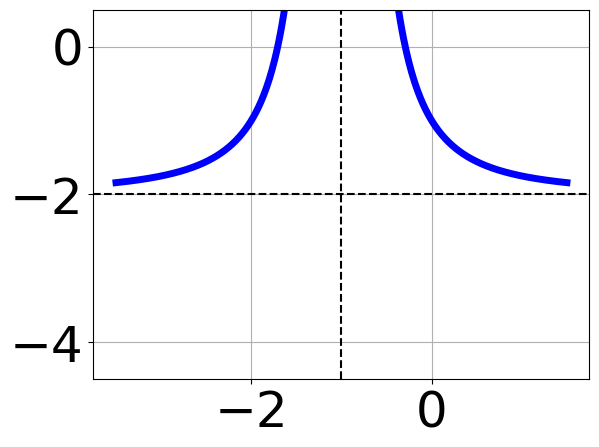
\includegraphics[width=0.5\textwidth]{../Figures/rationalGraphToEquationC.png}
\end{center}


The solution is \( f(x) = \frac{1}{(x + 1)^2} - 2 \), which is option D.\begin{enumerate}[label=\Alph*.]
\item \( f(x) = \frac{-1}{(x - 1)^2} - 2 \)

Corresponds to using the general form $f(x) = \frac{a}{(x+h)^2}+k$ and the opposite leading coefficient.
\item \( f(x) = \frac{-1}{x - 1} - 2 \)

Corresponds to thinking the graph was a shifted version of $\frac{1}{x}$, using the general form $f(x) = \frac{a}{(x+h)^2}+k$, and the opposite leading coefficient.
\item \( f(x) = \frac{1}{x + 1} - 2 \)

Corresponds to thinking the graph was a shifted version of $\frac{1}{x}$.
\item \( f(x) = \frac{1}{(x + 1)^2} - 2 \)

This is the correct option.
\item \( \text{None of the above} \)

This corresponds to believing the vertex of the graph was not correct.
\end{enumerate}

\textbf{General Comment:} Remember that the general form of a basic rational equation is $ f(x) = \frac{a}{(x-h)^n} + k$, where $a$ is the leading coefficient (and in this case, we assume is either $1$ or $-1$), $n$ is the degree (in this case, either $1$ or $2$), and $(h, k)$ is the intersection of the asymptotes.
}
\litem{
Determine the domain of the function below.
\[ f(x) = \frac{3}{12x^{2} -29 x + 15} \]The solution is \( \text{All Real numbers except } x = 0.750 \text{ and } x = 1.667. \), which is option C.\begin{enumerate}[label=\Alph*.]
\item \( \text{All Real numbers except } x = a, \text{ where } a \in [11.1, 14] \)

All Real numbers except $x = 12.000$, which corresponds to removing a distractor value from the denominator.
\item \( \text{All Real numbers except } x = a, \text{ where } a \in [-1.9, 1.2] \)

All Real numbers except $x = 0.750$, which corresponds to removing only 1 value from the denominator.
\item \( \text{All Real numbers except } x = a \text{ and } x = b, \text{ where } a \in [-1.9, 1.2] \text{ and } b \in [1.3, 3.6] \)

All Real numbers except $x = 0.750$ and $x = 1.667$, which is the correct option.
\item \( \text{All Real numbers.} \)

This corresponds to thinking the denominator has complex roots or that rational functions have a domain of all Real numbers.
\item \( \text{All Real numbers except } x = a \text{ and } x = b, \text{ where } a \in [11.1, 14] \text{ and } b \in [12.8, 15.3] \)

All Real numbers except $x = 12.000$ and $x = 15.000$, which corresponds to not factoring the denominator correctly.
\end{enumerate}

\textbf{General Comment:} Recall that dividing by zero is not a real number. Therefore the domain is all real numbers \textbf{except} those that make the denominator 0.
}
\litem{
Choose the graph of the equation below.
\[ f(x) = \frac{1}{(x + 2)^2} + 1 \]The solution is the graph below, which is option E.
    \begin{center}
        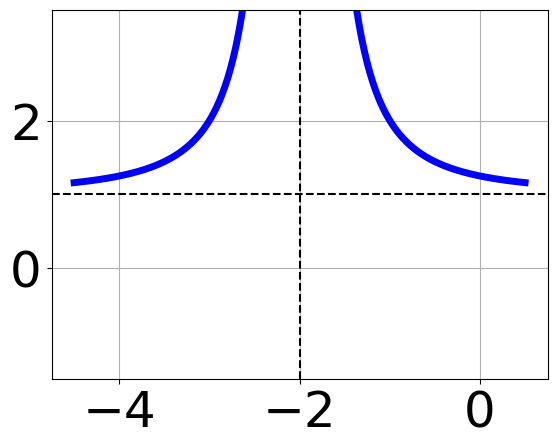
\includegraphics[width=0.3\textwidth]{../Figures/rationalEquationToGraphEC.png}
    \end{center}\begin{enumerate}[label=\Alph*.]
\begin{multicols}{2}
\item 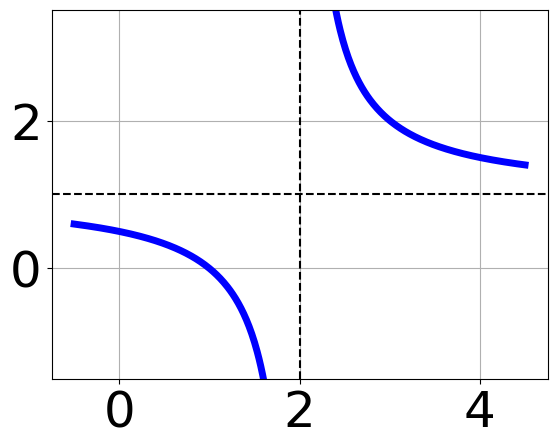
\includegraphics[width = 0.3\textwidth]{../Figures/rationalEquationToGraphAC.png}
\item 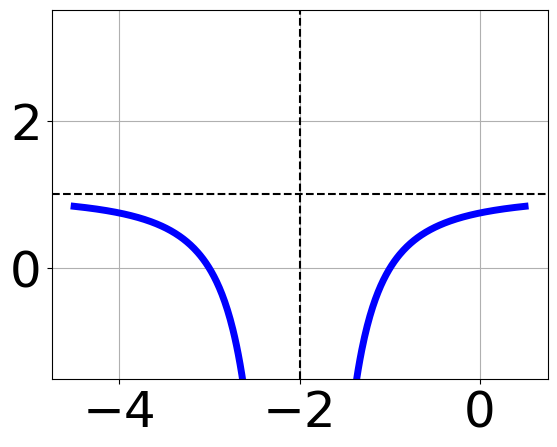
\includegraphics[width = 0.3\textwidth]{../Figures/rationalEquationToGraphBC.png}
\item 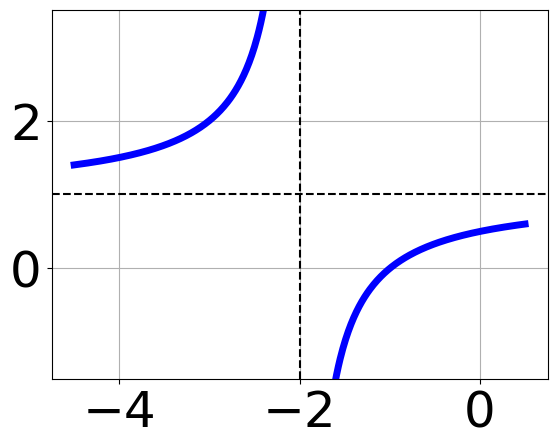
\includegraphics[width = 0.3\textwidth]{../Figures/rationalEquationToGraphCC.png}
\item 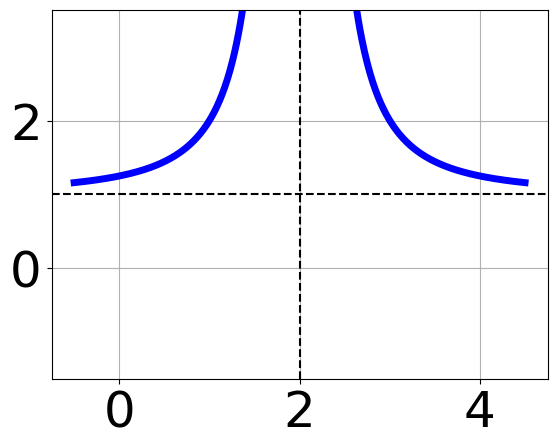
\includegraphics[width = 0.3\textwidth]{../Figures/rationalEquationToGraphDC.png}
\end{multicols}\item None of the above.\end{enumerate}
\textbf{General Comment:} Remember that the general form of a basic rational equation is $ f(x) = \frac{a}{(x-h)^n} + k$, where $a$ is the leading coefficient (and in this case, we assume is either $1$ or $-1$), $n$ is the degree (in this case, either $1$ or $2$), and $(h, k)$ is the intersection of the asymptotes.
}
\litem{
Solve the rational equation below. Then, choose the interval(s) that the solution(s) belongs to.
\[ \frac{2x}{-7x -7} + \frac{-2x^{2}}{49x^{2} +98 x + 49} = \frac{-5}{-7x -7} \]The solution is \( \text{There are two solutions: } x = -1.928 \text{ and } x = -1.135 \), which is option C.\begin{enumerate}[label=\Alph*.]
\item \( x_1 \in [-2.08, -1.92] \text{ and } x_2 \in [-1.06,-0.56] \)


\item \( x \in [-1.07,-0.9] \)


\item \( x_1 \in [-2.08, -1.92] \text{ and } x_2 \in [-1.23,-1.13] \)

* $x = -1.928 \text{ and } x = -1.135$, which is the correct option.
\item \( \text{All solutions lead to invalid or complex values in the equation.} \)


\item \( x \in [-1.4,-1.1] \)


\end{enumerate}

\textbf{General Comment:} Distractors are different based on the number of solutions. Remember that after solving, we need to make sure our solution does not make the original equation divide by zero!
}
\litem{
Solve the rational equation below. Then, choose the interval(s) that the solution(s) belongs to.
\[ \frac{-4}{8x -6} + 9 = \frac{9}{64x -48} \]The solution is \( x = 0.821 \), which is option A.\begin{enumerate}[label=\Alph*.]
\item \( x \in [-0.18,1.82] \)

* $x = 0.821$, which is the correct option.
\item \( x_1 \in [-2.68, 0.32] \text{ and } x_2 \in [0.55,0.83] \)

$x = -0.679 \text{ and } x = 0.821$, which corresponds to getting the correct solution and believing there should be a second solution to the equation.
\item \( x_1 \in [-0.18, 2.82] \text{ and } x_2 \in [0.84,1.26] \)

$x = 0.821 \text{ and } x = 0.931$, which corresponds to getting the correct solution and believing there should be a second solution to the equation.
\item \( \text{All solutions lead to invalid or complex values in the equation.} \)

This corresponds to thinking $x = 0.821$ leads to dividing by zero in the original equation, which it does not.
\item \( x \in [-2.68,0.32] \)

$x = -0.679$, which corresponds to not distributing the factor $8x -6$ correctly when trying to eliminate the fraction.
\end{enumerate}

\textbf{General Comment:} Distractors are different based on the number of solutions. Remember that after solving, we need to make sure our solution does not make the original equation divide by zero!
}
\end{enumerate}

\end{document}